% Options for packages loaded elsewhere
\PassOptionsToPackage{unicode}{hyperref}
\PassOptionsToPackage{hyphens}{url}
%
\documentclass[
  11pt,
]{article}
\usepackage{amsmath,amssymb}
\usepackage{lmodern}
\usepackage{setspace}
\usepackage{iftex}
\ifPDFTeX
  \usepackage[T1]{fontenc}
  \usepackage[utf8]{inputenc}
  \usepackage{textcomp} % provide euro and other symbols
\else % if luatex or xetex
  \usepackage{unicode-math}
  \defaultfontfeatures{Scale=MatchLowercase}
  \defaultfontfeatures[\rmfamily]{Ligatures=TeX,Scale=1}
\fi
% Use upquote if available, for straight quotes in verbatim environments
\IfFileExists{upquote.sty}{\usepackage{upquote}}{}
\IfFileExists{microtype.sty}{% use microtype if available
  \usepackage[]{microtype}
  \UseMicrotypeSet[protrusion]{basicmath} % disable protrusion for tt fonts
}{}
\makeatletter
\@ifundefined{KOMAClassName}{% if non-KOMA class
  \IfFileExists{parskip.sty}{%
    \usepackage{parskip}
  }{% else
    \setlength{\parindent}{0pt}
    \setlength{\parskip}{6pt plus 2pt minus 1pt}}
}{% if KOMA class
  \KOMAoptions{parskip=half}}
\makeatother
\usepackage{xcolor}
\usepackage[margin=1in]{geometry}
\usepackage{color}
\usepackage{fancyvrb}
\newcommand{\VerbBar}{|}
\newcommand{\VERB}{\Verb[commandchars=\\\{\}]}
\DefineVerbatimEnvironment{Highlighting}{Verbatim}{commandchars=\\\{\}}
% Add ',fontsize=\small' for more characters per line
\usepackage{framed}
\definecolor{shadecolor}{RGB}{248,248,248}
\newenvironment{Shaded}{\begin{snugshade}}{\end{snugshade}}
\newcommand{\AlertTok}[1]{\textcolor[rgb]{0.94,0.16,0.16}{#1}}
\newcommand{\AnnotationTok}[1]{\textcolor[rgb]{0.56,0.35,0.01}{\textbf{\textit{#1}}}}
\newcommand{\AttributeTok}[1]{\textcolor[rgb]{0.77,0.63,0.00}{#1}}
\newcommand{\BaseNTok}[1]{\textcolor[rgb]{0.00,0.00,0.81}{#1}}
\newcommand{\BuiltInTok}[1]{#1}
\newcommand{\CharTok}[1]{\textcolor[rgb]{0.31,0.60,0.02}{#1}}
\newcommand{\CommentTok}[1]{\textcolor[rgb]{0.56,0.35,0.01}{\textit{#1}}}
\newcommand{\CommentVarTok}[1]{\textcolor[rgb]{0.56,0.35,0.01}{\textbf{\textit{#1}}}}
\newcommand{\ConstantTok}[1]{\textcolor[rgb]{0.00,0.00,0.00}{#1}}
\newcommand{\ControlFlowTok}[1]{\textcolor[rgb]{0.13,0.29,0.53}{\textbf{#1}}}
\newcommand{\DataTypeTok}[1]{\textcolor[rgb]{0.13,0.29,0.53}{#1}}
\newcommand{\DecValTok}[1]{\textcolor[rgb]{0.00,0.00,0.81}{#1}}
\newcommand{\DocumentationTok}[1]{\textcolor[rgb]{0.56,0.35,0.01}{\textbf{\textit{#1}}}}
\newcommand{\ErrorTok}[1]{\textcolor[rgb]{0.64,0.00,0.00}{\textbf{#1}}}
\newcommand{\ExtensionTok}[1]{#1}
\newcommand{\FloatTok}[1]{\textcolor[rgb]{0.00,0.00,0.81}{#1}}
\newcommand{\FunctionTok}[1]{\textcolor[rgb]{0.00,0.00,0.00}{#1}}
\newcommand{\ImportTok}[1]{#1}
\newcommand{\InformationTok}[1]{\textcolor[rgb]{0.56,0.35,0.01}{\textbf{\textit{#1}}}}
\newcommand{\KeywordTok}[1]{\textcolor[rgb]{0.13,0.29,0.53}{\textbf{#1}}}
\newcommand{\NormalTok}[1]{#1}
\newcommand{\OperatorTok}[1]{\textcolor[rgb]{0.81,0.36,0.00}{\textbf{#1}}}
\newcommand{\OtherTok}[1]{\textcolor[rgb]{0.56,0.35,0.01}{#1}}
\newcommand{\PreprocessorTok}[1]{\textcolor[rgb]{0.56,0.35,0.01}{\textit{#1}}}
\newcommand{\RegionMarkerTok}[1]{#1}
\newcommand{\SpecialCharTok}[1]{\textcolor[rgb]{0.00,0.00,0.00}{#1}}
\newcommand{\SpecialStringTok}[1]{\textcolor[rgb]{0.31,0.60,0.02}{#1}}
\newcommand{\StringTok}[1]{\textcolor[rgb]{0.31,0.60,0.02}{#1}}
\newcommand{\VariableTok}[1]{\textcolor[rgb]{0.00,0.00,0.00}{#1}}
\newcommand{\VerbatimStringTok}[1]{\textcolor[rgb]{0.31,0.60,0.02}{#1}}
\newcommand{\WarningTok}[1]{\textcolor[rgb]{0.56,0.35,0.01}{\textbf{\textit{#1}}}}
\usepackage{longtable,booktabs,array}
\usepackage{calc} % for calculating minipage widths
% Correct order of tables after \paragraph or \subparagraph
\usepackage{etoolbox}
\makeatletter
\patchcmd\longtable{\par}{\if@noskipsec\mbox{}\fi\par}{}{}
\makeatother
% Allow footnotes in longtable head/foot
\IfFileExists{footnotehyper.sty}{\usepackage{footnotehyper}}{\usepackage{footnote}}
\makesavenoteenv{longtable}
\usepackage{graphicx}
\makeatletter
\def\maxwidth{\ifdim\Gin@nat@width>\linewidth\linewidth\else\Gin@nat@width\fi}
\def\maxheight{\ifdim\Gin@nat@height>\textheight\textheight\else\Gin@nat@height\fi}
\makeatother
% Scale images if necessary, so that they will not overflow the page
% margins by default, and it is still possible to overwrite the defaults
% using explicit options in \includegraphics[width, height, ...]{}
\setkeys{Gin}{width=\maxwidth,height=\maxheight,keepaspectratio}
% Set default figure placement to htbp
\makeatletter
\def\fps@figure{htbp}
\makeatother
\setlength{\emergencystretch}{3em} % prevent overfull lines
\providecommand{\tightlist}{%
  \setlength{\itemsep}{0pt}\setlength{\parskip}{0pt}}
\setcounter{secnumdepth}{-\maxdimen} % remove section numbering
\usepackage{float}
\floatplacement{figure}{ht}
\usepackage[section]{placeins}
\usepackage{longtable}
\usepackage{hyperref}
\hypersetup{colorlinks = true, linkcolor = blue, urlcolor = blue}
\widowpenalty10000
\clubpenalty10000
\usepackage[page,header]{appendix}
\usepackage{titletoc}
\usepackage{tocloft}
\usepackage{makecell}
\ifLuaTeX
  \usepackage{selnolig}  % disable illegal ligatures
\fi
\IfFileExists{bookmark.sty}{\usepackage{bookmark}}{\usepackage{hyperref}}
\IfFileExists{xurl.sty}{\usepackage{xurl}}{} % add URL line breaks if available
\urlstyle{same} % disable monospaced font for URLs
\hypersetup{
  pdftitle={Lecture: Applied Bayesian Statistics Using Stan: Basics},
  pdfauthor={Denis Cohen},
  hidelinks,
  pdfcreator={LaTeX via pandoc}}

\title{Lecture: Applied Bayesian Statistics Using Stan: Basics}
\author{Denis Cohen\footnote{Mannheim Centre for European Social Research, University of Mannheim, 68131 Mannheim, Germany. \href{mailto:denis.cohen@uni-mannheim.de}{\nolinkurl{denis.cohen@uni-mannheim.de}}.}}
\date{}

\begin{document}
\maketitle

\setstretch{1.5}
\hypertarget{stan}{%
\subsection{Stan}\label{stan}}

\hypertarget{what-is-stan}{%
\subsubsection{What is Stan?}\label{what-is-stan}}

In the words of the developers:

``Stan is a state-of-the-art platform for statistical modeling and high-performance statistical computation. Thousands of users rely on Stan for statistical modeling, data analysis, and prediction in the social, biological, and physical sciences, engineering, and business.

Users specify log density functions in Stan's probabilistic programming language and get:

\begin{itemize}
\tightlist
\item
  full Bayesian statistical inference with MCMC sampling (NUTS, HMC)
\item
  approximate Bayesian inference with variational inference (ADVI)
\item
  penalized maximum likelihood estimation with optimization (L-BFGS)
\end{itemize}

Source: \url{https://mc-stan.org/}

\hypertarget{why-stan}{%
\subsubsection{Why Stan?}\label{why-stan}}

\begin{itemize}
\tightlist
\item
  Open-source software
\item
  Fast and stable algorithms
\item
  High flexibility with few limitations
\item
  Extensive documentation

  \begin{itemize}
  \tightlist
  \item
    \href{https://mc-stan.org/docs/2_19/stan-users-guide/index.html}{User's Guide}
  \item
    \href{https://mc-stan.org/docs/2_19/reference-manual/index.html}{Language Reference Manual}
  \item
    \href{https://mc-stan.org/docs/2_19/functions-reference/index.html}{Language Functions Reference}
  \end{itemize}
\item
  Highly transparent development process; see \href{https://github.com/stan-dev/stan}{Stan Development Repository on Github}
\item
  Very responsive \href{https://mc-stan.org/about/team/}{Development Team}
\item
  Large and active community in the \href{https://discourse.mc-stan.org/}{Stan Forums} and \href{https://stackoverflow.com/questions/tagged/stan}{Stack OVerflow}
\item
  Increasing number of \href{https://mc-stan.org/users/documentation/case-studies.html}{case studies}, \href{https://mc-stan.org/users/documentation/tutorials.html}{tutorials}, \href{https://mc-stan.org/users/documentation/external.html}{papers and textbooks}
\item
  Compatibility with various editor for syntax highlighting, formatting, and checking (incl.~\href{https://www.rstudio.com/}{RStudio} and \href{https://www.gnu.org/software/emacs/}{Emacs})
\end{itemize}

\hypertarget{stan-interfaces}{%
\subsubsection{Stan interfaces}\label{stan-interfaces}}

\begin{itemize}
\tightlist
\item
  RStan (R)
\item
  PyStan (Python)
\item
  CmdStan (shell, command-line terminal)
\item
  MatlabStan (MATLAB)
\item
  Stan.jl (Julia)
\item
  StataStan (Stata)
\item
  MathematicaStan (Mathematica)
\item
  ScalaStan (Scala)
\end{itemize}

\hypertarget{some-r-packages}{%
\subsubsection{(Some) R packages}\label{some-r-packages}}

\begin{itemize}
\tightlist
\item
  \href{https://cran.r-project.org/package=rstan}{\textbf{rstan}}: General R Interface to Stan
\item
  \href{https://cran.r-project.org/package=shinystan}{\textbf{shinystan}}: Interactive Visual and Numerical Diagnostics and Posterior Analysis for Bayesian Models
\item
  \href{https://cran.r-project.org/web/packages/bayesplot/index.html}{\textbf{bayesplot}}: Plotting functions for posterior analysis, model checking, and MCMC diagnostics.
\item
  \href{https://cran.r-project.org/package=brms}{\textbf{brms}}: Bayesian Regression Models using `Stan', covering a growing number of model types
\item
  \href{https://cran.r-project.org/package=rstanarm}{\textbf{rstanarm}}: Bayesian Applied Regression Modeling via Stan, with an emphasis on hierarchical/multilevel models
\item
  \href{https://cran.r-project.org/package=edstan}{\textbf{edstan}}: Stan Models for Item Response Theory
\item
  \href{https://cran.r-project.org/package=rstantools}{\textbf{rstantools}}: Tools for Developing R Packages Interfacing with `Stan'
\end{itemize}

\hypertarget{caveat-reproducibility}{%
\subsubsection{Caveat: Reproducibility}\label{caveat-reproducibility}}

Under what conditions are estimates reproducible? See \href{https://mc-stan.org/docs/2_19/reference-manual/reproducibility-chapter.html}{Stan Reference Manual}, Section 19:

\begin{itemize}
\tightlist
\item
  Stan version
\item
  Stan interface (RStan, PyStan, CmdStan) and version, plus version of interface language (R, Python, shell)
\item
  versions of included libraries (Boost and Eigen)
\item
  operating system version
\item
  computer hardware including CPU, motherboard and memory
\item
  C++ compiler, including version, compiler flags, and linked libraries
\item
  same configuration of call to Stan, including random seed, chain ID, initialization and data
\end{itemize}

\hypertarget{bayesian-workflow}{%
\subsection{Bayesian workflow}\label{bayesian-workflow}}

\hypertarget{a-quick-overview}{%
\subsubsection{A quick overview}\label{a-quick-overview}}

\hypertarget{the-short-version}{%
\paragraph{The short version}\label{the-short-version}}

\begin{enumerate}
\def\labelenumi{\arabic{enumi}.}
\tightlist
\item
  \textbf{Specification}: Specify the full probability model

  \begin{itemize}
  \tightlist
  \item
    data
  \item
    likelihood
  \item
    priors
  \end{itemize}
\item
  \textbf{Model Building}: Translate the model into code
\item
  \textbf{Validation}: Validate the model with fake data
\item
  \textbf{Fitting}: Fit the model to actual data
\item
  \textbf{Diagnosis}: Check generic and algorithm-specific diagnostics to assess convergence
\item
  Posterior Predictive Checks
\item
  Model Comparison
\end{enumerate}

Source: \href{http://nbviewer.jupyter.org/github/QuantEcon/QuantEcon.notebooks/blob/master/IntroToStan_basics_workflow.ipynb}{Jim Savage (2016) A quick-start introduction to Stan for economists. A QuantEcon Notebook.}

\hypertarget{the-long-version}{%
\paragraph{The long version}\label{the-long-version}}

\begin{center}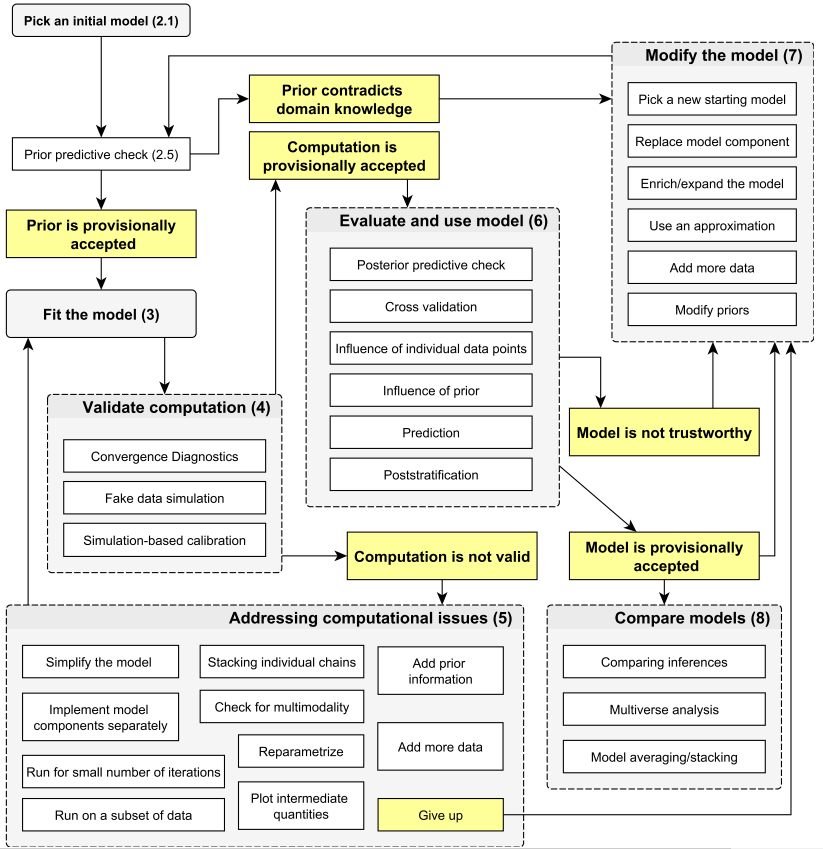
\includegraphics[width=0.9\linewidth]{images/workflow} \end{center}

Source: \href{https://arxiv.org/abs/2011.01808}{Gelman, A., Vehtari, A., Simpson, D., Margossian, C. C., Carpenter, B., Yao, Y., Kennedy, L., Gabry, J., Bürkner, P. C., \& Modrák, M. (2020). Bayesian workflow.}

\hypertarget{specification-linear-model}{%
\subsection{Specification (linear model)}\label{specification-linear-model}}

\hypertarget{reminder-equivalent-notations}{%
\subsubsection{Reminder: Equivalent notations}\label{reminder-equivalent-notations}}

\begin{enumerate}
\def\labelenumi{\arabic{enumi}.}
\tightlist
\item
  Scalar form: \[y_i = \beta_1 x_{i1} + \beta_2 x_{i2} + \beta_3 x_{i3} + \epsilon_i \text{ for all } i=1,...,N\]
\item
  Row-vector form: \[y_i = \mathbf{x_i^{\prime}} \mathbf{\beta} + \epsilon_i  \text{ for all } i=1,...,N\]
\item
  Column-vector form: \[\mathbf{y} = \beta_1 \mathbf{x_{1}} + \beta_2 \mathbf{x_{2}} + \beta_3 \mathbf{x_{3}} \mathbf{\epsilon}\]
\item
  Matrix form: \[\mathbf{y = X \beta + \epsilon}\]
\end{enumerate}

\hypertarget{example-linear-model}{%
\subsubsection{Example: Linear model}\label{example-linear-model}}

Our knowledge of generalized linear models gives us \emph{almost} everything we need!

\hypertarget{probability-model-for-the-data}{%
\subsubsection{Probability model for the data}\label{probability-model-for-the-data}}

First, let's recap the three parts of every GLM in the context of the linear model:

\begin{itemize}
\tightlist
\item
  Family: \(\mathbf{y} \sim \text{Normal}(\eta, \sigma)\)
\item
  (Inverse) link function: \(\mathbf{y^{\ast}} = \text{id}(\eta) = \eta\)
\item
  Linear component: \(\eta = \mathbf{X} \beta\)
\end{itemize}

The \emph{family} specifies the probability model (a.k.a. likelihood, data-generating process, or generative model) for the \emph{data}: The fundamental assumption of the linear model is that every observation \(y_i\) is a realization from a normal pdf with location parameter (mean) \(\eta_i\) and constant scale parameter (variance) \(\sigma^2\).

\emph{Note:} Mimicking the convention in both R and Stan, we parameterize the normal distribution in terms of its mean and \emph{standard deviation} (not variance)!

\hypertarget{known-and-unknown-quantities}{%
\subsubsection{Known and unknown quantities}\label{known-and-unknown-quantities}}

\begin{itemize}
\tightlist
\item
  Parameters (unknown, random quantities):

  \begin{itemize}
  \tightlist
  \item
    \(\beta\), the coefficient vector
  \item
    \(\sigma\), the scale parameter of the normal
  \item
    \(\eta\), the location parameter of the normal
  \end{itemize}
\item
  Data (known, fixed quantities):

  \begin{itemize}
  \tightlist
  \item
    \(\mathbf{y}\), the outcome vector
  \item
    \(\mathbf{X}\), the design matrix
  \item
    the dimensions of \(\mathbf{y}_{N \times 1}\) and \(\mathbf{X}_{N \times K}\)
  \item
    the dimensions of \(\beta_{K \times 1}\), \(\sigma\) (a scalar), and \(\eta_{N \times 1}\)
  \end{itemize}
\end{itemize}

\hypertarget{priors}{%
\subsubsection{Priors}\label{priors}}

What is still missing are prior distributions for the unknown quantities.

Here, we have quite some discretion. There are few rules we must adhere to:

\begin{itemize}
\tightlist
\item
  Our \(\beta\)'s have unconstrained support (though by far not all value ranges may be reasonable!)
\item
  The scale parameter \(\sigma\) cannot be negative
\end{itemize}

Here, we will opt for a convenience solution and specify weakly informative zero-mean normal priors for the \(\beta\)'s and a weakly informative half-Cauchy prior for \(\sigma\):

\begin{itemize}
\tightlist
\item
  \(\beta \sim \text{N}(0, 10)\)
\item
  \(\sigma \sim \text{Cauchy}^{+}(0, 5)\)
\end{itemize}

\begin{center}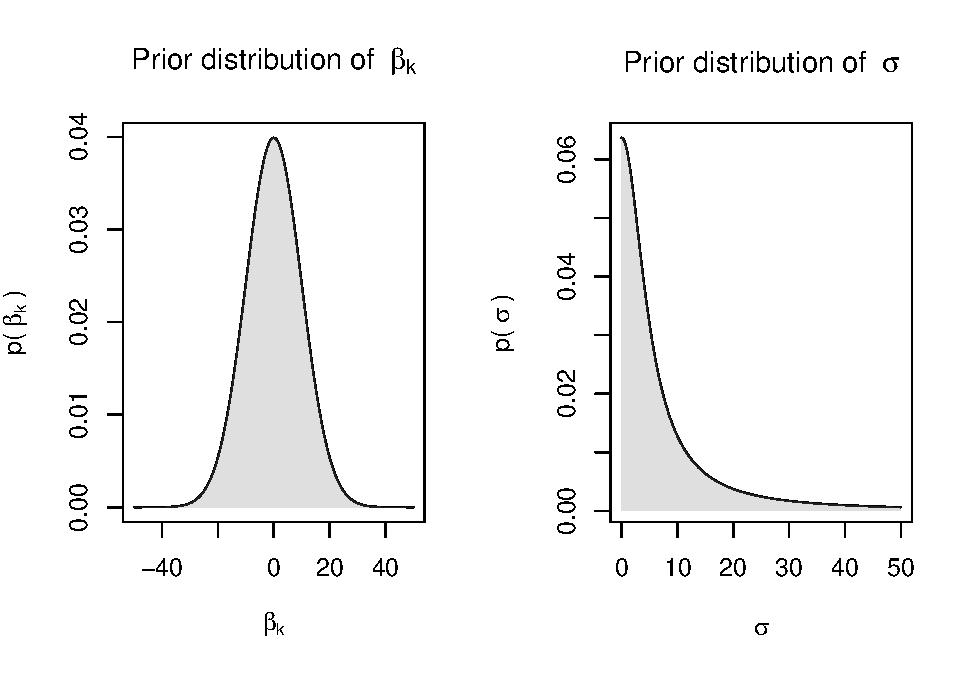
\includegraphics{04-lec_files/figure-latex/prior-viz-1} \end{center}

\hypertarget{model-building}{%
\subsection{Model building}\label{model-building}}

\hypertarget{stan-program-blocks}{%
\subsubsection{Stan Program Blocks}\label{stan-program-blocks}}

\begin{enumerate}
\def\labelenumi{\arabic{enumi}.}
\tightlist
\item
  Functions: Declare user written functions
\item
  \textbf{Data}: Declare all known quantities
\item
  Transformed Data: Transform declared data inputs (once)
\item
  \textbf{Parameters}: Declare all unknown quantities
\item
  Transformed Parameters: Transform declared parameters (each step, each iteration)
\item
  \textbf{Model}: Transform parameters, specify prior distributions and likelihoods
\item
  Generated Quantities (each iteration)
\end{enumerate}

\hypertarget{program-blocks}{%
\subsubsection{Program Blocks}\label{program-blocks}}

\begin{center}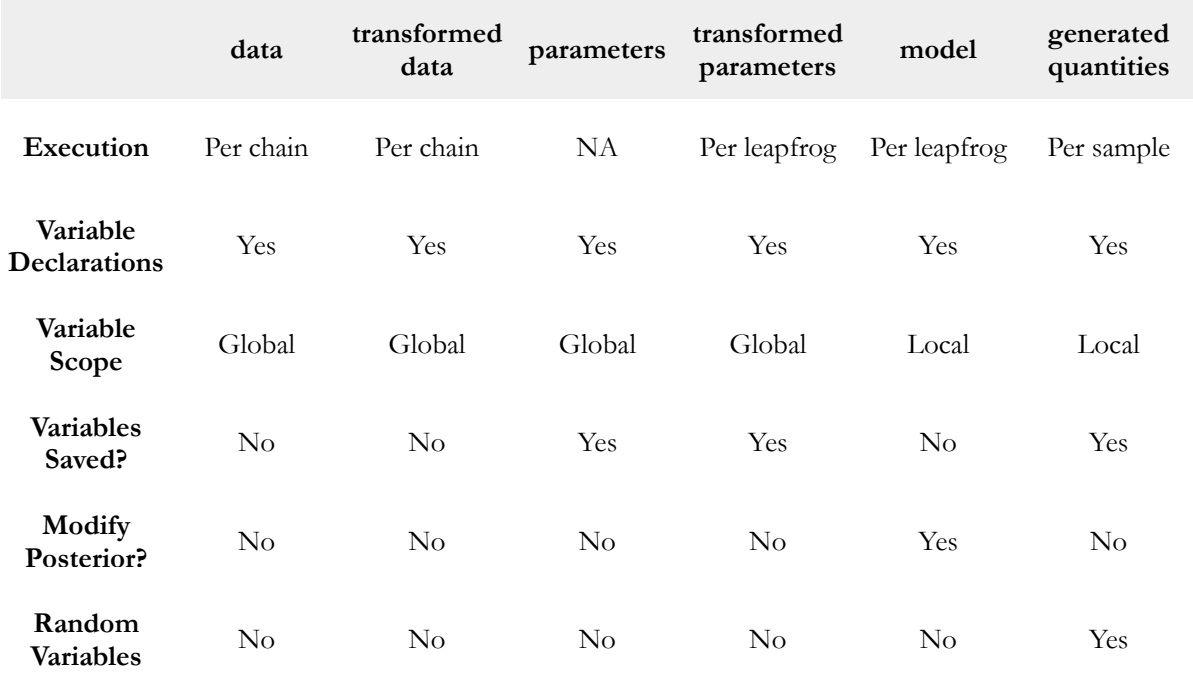
\includegraphics[width=0.72\linewidth]{images/blocks} \end{center}

Source: \url{http://mlss2014.hiit.fi/mlss_files/2-stan.pdf}

\hypertarget{script-for-a-stan-program}{%
\subsubsection{Script for a Stan program}\label{script-for-a-stan-program}}

\emph{Writing scripts for Stan programs}

\begin{itemize}
\tightlist
\item
  Start with a blank script in your preferred code editor and save it as ``lm.stan'' .
\item
  This will enable syntax highlighting, formatting, and checking in RStudio and Emacs.
\item
  Alternatively, you can save your model as a single character string in R (with some drawbacks).
\end{itemize}

\emph{Style guide}

\begin{itemize}
\tightlist
\item
  There is a \href{https://mc-stan.org/docs/2_26/stan-users-guide/stan-program-style-guide.html}{style guide}. Some recommendations:

  \begin{itemize}
  \tightlist
  \item
    consistency
  \item
    lines should not exceed 80 characters
  \item
    lowercase variables, words separated by underscores
  \item
    like R: space around operators: \texttt{y\ \textasciitilde{}\ normal(...)}, \texttt{x\ =\ (1\ +\ 2)\ *\ 3}
  \item
    spaces after commas are optional: \texttt{y{[}m,n{]}\ \textasciitilde{}\ normal(0,1)} or \texttt{y{[}m,\ n{]}\ \textasciitilde{}\ normal(0,\ 1)}
  \end{itemize}
\item
  Always make sure to end your script with a blank line.
\item
  You must use a delimiter to finish lines: \texttt{;}.
\item
  \texttt{//\ this\ is\ a\ comment}
\end{itemize}

\hypertarget{data-block}{%
\subsubsection{Data block}\label{data-block}}

Declare all known quantities, including data types, dimensions, and constraints:

\begin{itemize}
\tightlist
\item
  \(\mathbf{y}_{N \times 1}\)
\item
  \(\mathbf{X}_{N \times K}\)
\end{itemize}

\begin{Shaded}
\begin{Highlighting}[]
\KeywordTok{data}\NormalTok{ \{}
  \DataTypeTok{int}\NormalTok{\textless{}}\KeywordTok{lower}\NormalTok{=}\DecValTok{1}\NormalTok{\textgreater{} N; }\CommentTok{// num. observations}
  \DataTypeTok{int}\NormalTok{\textless{}}\KeywordTok{lower}\NormalTok{=}\DecValTok{1}\NormalTok{\textgreater{} K; }\CommentTok{// num. predictors}
  \DataTypeTok{matrix}\NormalTok{[N, K] x; }\CommentTok{// model matrix}
  \DataTypeTok{vector}\NormalTok{[N] y;    }\CommentTok{// outcome vector}
\NormalTok{\}}
\end{Highlighting}
\end{Shaded}

\hypertarget{parameters-block}{%
\subsubsection{Parameters block}\label{parameters-block}}

Declare unknown `base' quantities, including storage types, dimensions, and constraints:

\begin{itemize}
\tightlist
\item
  \(\beta\), the coefficient vector
\item
  \(\sigma\), the scale parameter of the normal
\end{itemize}

\begin{Shaded}
\begin{Highlighting}[]
\KeywordTok{parameters}\NormalTok{ \{}
\NormalTok{  ... declarations ...}
\NormalTok{\}}
\end{Highlighting}
\end{Shaded}

\hypertarget{transformed-parameters-block}{%
\subsubsection{Transformed parameters block}\label{transformed-parameters-block}}

Declare and specify unknown transformed quantities, including storage types, dimensions, and constraints:

\begin{itemize}
\tightlist
\item
  \(\eta = \mathbf{X} \beta\), the linear prediction
\end{itemize}

\begin{Shaded}
\begin{Highlighting}[]
\KeywordTok{transformed parameters}\NormalTok{ \{}
\NormalTok{  ... declarations ... statements ....}
\NormalTok{\}}
\end{Highlighting}
\end{Shaded}

\hypertarget{model-block}{%
\subsubsection{Model block}\label{model-block}}

Declare and specify local variables (optional) and specify sampling statements:

\begin{itemize}
\tightlist
\item
  \(\beta_k \sim \text{Normal}(0, 10) \text{ for k = 1,...,K}\)
\item
  \(\sigma \sim \text{Cauchy}^{+}(0, 5)\)
\item
  \(\mathbf{y} \sim \text{Normal}(\eta, \sigma)\)
\end{itemize}

\begin{Shaded}
\begin{Highlighting}[]
\KeywordTok{model}\NormalTok{ \{}
  \CommentTok{// priors}
\NormalTok{  ... statements ...}
  
  \CommentTok{// log{-}likelihood}
\NormalTok{  ... statements ...}
\NormalTok{\}}
\end{Highlighting}
\end{Shaded}

\hypertarget{writing-stan-programs-in-r}{%
\subsubsection{Writing Stan programs in R}\label{writing-stan-programs-in-r}}

\begin{itemize}
\tightlist
\item
  You can supply Stan programs as a character string in R
\item
  Downsides:

  \begin{itemize}
  \tightlist
  \item
    No syntax highlighting, formatting, and checking
  \item
    Must use double quotation marks \texttt{"} around the string to avoid that the \href{https://mc-stan.org/docs/2_26/functions-reference/transposition-operator.html}{transposition operator} \texttt{\textquotesingle{}} breaks the string
  \end{itemize}
\item
  Upsides: Works with the interactive \texttt{learnr} tutorials in our workshop!
\end{itemize}

\begin{Shaded}
\begin{Highlighting}[]
\CommentTok{\# Save as character}
\NormalTok{lm\_code }\OtherTok{\textless{}{-}} 
\StringTok{"data \{}
\StringTok{  int\textless{}lower=1\textgreater{} N; // num. observations}
\StringTok{  int\textless{}lower=1\textgreater{} K; // num. predictors}
\StringTok{  matrix[N, K] x; // design matrix}
\StringTok{  vector[N] y;    // outcome vector}
\StringTok{\}}

\StringTok{parameters \{}
\StringTok{  vector[K] beta;      // coef vector}
\StringTok{  real\textless{}lower=0\textgreater{} sigma; // scale parameter}
\StringTok{\}}

\StringTok{transformed parameters \{}
\StringTok{  vector[N] eta;  // declare lin. pred.}
\StringTok{  eta = x * beta; // assign lin. pred.}
\StringTok{\}}

\StringTok{model \{}
\StringTok{  // priors}
\StringTok{  target += normal\_lpdf(beta | 0, 10);  // priors for beta}
\StringTok{  target += cauchy\_lpdf(sigma | 0, 5);  // prior for sigma}
\StringTok{  }
\StringTok{  // log{-}likelihood}
\StringTok{  target += normal\_lpdf(y | eta, sigma); // likelihood}
\StringTok{\}"}

\CommentTok{\# Write to script}
\FunctionTok{writeLines}\NormalTok{(lm\_code, }\AttributeTok{con =} \StringTok{"lm.stan"}\NormalTok{)}
\end{Highlighting}
\end{Shaded}

\hypertarget{validation}{%
\subsection{Validation}\label{validation}}

\hypertarget{simulate-the-data-generating-process-in-r}{%
\subsubsection{Simulate the data-generating process in R}\label{simulate-the-data-generating-process-in-r}}

\hypertarget{setup-and-compilation}{%
\subsubsection{Setup and compilation}\label{setup-and-compilation}}

\begin{Shaded}
\begin{Highlighting}[]
\DocumentationTok{\#\# Setup}
\FunctionTok{library}\NormalTok{(rstan)}
\FunctionTok{rstan\_options}\NormalTok{(}\AttributeTok{auto\_write =} \ConstantTok{TRUE}\NormalTok{)             }\CommentTok{\# avoid recompilation of models}
\FunctionTok{options}\NormalTok{(}\AttributeTok{mc.cores =}\NormalTok{ parallel}\SpecialCharTok{::}\FunctionTok{detectCores}\NormalTok{())  }\CommentTok{\# parallelize across all CPUs}

\DocumentationTok{\#\# Data as list}
\NormalTok{standat\_val }\OtherTok{\textless{}{-}} \FunctionTok{list}\NormalTok{(}
  \AttributeTok{N =}\NormalTok{ N,}
  \AttributeTok{K =}\NormalTok{ K,}
  \AttributeTok{x =}\NormalTok{ x,}
  \AttributeTok{y =}\NormalTok{ y\_sim}
\NormalTok{)}

\DocumentationTok{\#\# C++ Compilation}
\NormalTok{lm\_mod }\OtherTok{\textless{}{-}}\NormalTok{ rstan}\SpecialCharTok{::}\FunctionTok{stan\_model}\NormalTok{(}\AttributeTok{model\_code =}\NormalTok{ lm\_code)}
\end{Highlighting}
\end{Shaded}

\hypertarget{estimation}{%
\subsubsection{Estimation}\label{estimation}}

\begin{Shaded}
\begin{Highlighting}[]
\NormalTok{lm\_val }\OtherTok{\textless{}{-}}\NormalTok{ rstan}\SpecialCharTok{::}\FunctionTok{sampling}\NormalTok{(}
\NormalTok{  lm\_mod,                     }\CommentTok{\# compiled model}
  \AttributeTok{data =}\NormalTok{ standat\_val,             }\CommentTok{\# data input}
  \AttributeTok{algorithm =} \StringTok{"NUTS"}\NormalTok{,         }\CommentTok{\# algorithm}
  \AttributeTok{control =} \FunctionTok{list}\NormalTok{(             }\CommentTok{\# control arguments}
    \AttributeTok{adapt\_delta =}\NormalTok{ .}\DecValTok{85}\NormalTok{),}
  \AttributeTok{save\_warmup =} \ConstantTok{FALSE}\NormalTok{,        }\CommentTok{\# discard warmup sims}
  \AttributeTok{sample\_file =} \ConstantTok{NULL}\NormalTok{,         }\CommentTok{\# no sample file}
  \AttributeTok{diagnostic\_file =} \ConstantTok{NULL}\NormalTok{,     }\CommentTok{\# no diagnostic file}
  \AttributeTok{pars =} \FunctionTok{c}\NormalTok{(}\StringTok{"beta"}\NormalTok{, }\StringTok{"sigma"}\NormalTok{),  }\CommentTok{\# select parameters}
  \AttributeTok{iter =}\NormalTok{ 2000L,               }\CommentTok{\# iter per chain}
  \AttributeTok{warmup =}\NormalTok{ 1000L,             }\CommentTok{\# warmup period}
  \AttributeTok{thin =}\NormalTok{ 2L,                  }\CommentTok{\# thinning factor}
  \AttributeTok{chains =}\NormalTok{ 2L,                }\CommentTok{\# num. chains}
  \AttributeTok{cores =}\NormalTok{ 2L,                 }\CommentTok{\# num. cores}
  \AttributeTok{seed =} \DecValTok{20210329}\NormalTok{)            }\CommentTok{\# seed}
\end{Highlighting}
\end{Shaded}

\hypertarget{output-summary}{%
\subsubsection{Output summary}\label{output-summary}}

\emph{Reminder:} Here are the `true' parameter values:

\begin{Shaded}
\begin{Highlighting}[]
\NormalTok{true\_pars }\OtherTok{\textless{}{-}} \FunctionTok{c}\NormalTok{(beta, sigma)}
\FunctionTok{names}\NormalTok{(true\_pars) }\OtherTok{\textless{}{-}} \FunctionTok{c}\NormalTok{(}\FunctionTok{paste0}\NormalTok{(}\StringTok{"beta["}\NormalTok{, }\DecValTok{1}\SpecialCharTok{:}\DecValTok{5}\NormalTok{, }\StringTok{"]"}\NormalTok{), }\StringTok{"sigma"}\NormalTok{)}
\NormalTok{true\_pars}
\end{Highlighting}
\end{Shaded}

\begin{verbatim}
##    beta[1]    beta[2]    beta[3]    beta[4]    beta[5]      sigma 
## -0.5243799 -1.1456866 -1.4379737  0.3127257  2.4365995  2.5000000
\end{verbatim}

And here are the estimates from our model:

\begin{Shaded}
\begin{Highlighting}[]
\NormalTok{lm\_val}
\end{Highlighting}
\end{Shaded}

\begin{verbatim}
## Inference for Stan model: 37c095a6cbe3e8a27908a77406b6b94d.
## 2 chains, each with iter=2000; warmup=1000; thin=2; 
## post-warmup draws per chain=500, total post-warmup draws=1000.
## 
##             mean se_mean   sd     2.5%      25%      50%      75%    97.5%
## beta[1]    -0.61    0.00 0.08    -0.78    -0.67    -0.61    -0.55    -0.45
## beta[2]    -1.05    0.00 0.08    -1.21    -1.11    -1.05    -1.00    -0.90
## beta[3]    -1.50    0.00 0.08    -1.66    -1.56    -1.50    -1.45    -1.34
## beta[4]     0.34    0.00 0.08     0.18     0.29     0.33     0.39     0.49
## beta[5]     2.50    0.00 0.09     2.32     2.44     2.50     2.56     2.66
## sigma       2.53    0.00 0.06     2.42     2.49     2.53     2.58     2.66
## lp__    -2367.19    0.07 1.94 -2371.89 -2368.19 -2366.81 -2365.79 -2364.58
##         n_eff Rhat
## beta[1]   925 1.00
## beta[2]   913 1.01
## beta[3]   875 1.00
## beta[4]   946 1.00
## beta[5]   851 1.00
## sigma     918 1.00
## lp__      678 1.00
## 
## Samples were drawn using NUTS(diag_e) at Fri Mar 26 13:55:16 2021.
## For each parameter, n_eff is a crude measure of effective sample size,
## and Rhat is the potential scale reduction factor on split chains (at 
## convergence, Rhat=1).
\end{verbatim}

\begin{itemize}
\tightlist
\item
  When comparing these estimates, the question is, of course, how much deviation should have us worried.
\item
  Deviations from a single validation run may be due to a circumstantial simulation of `extreme' outcome values when mimicking the data generating process.
\item
  \href{https://www.tandfonline.com/doi/abs/10.1198/106186006X136976}{Cook, Gelman, and Rubin (2006)} thus recommend running many replications of such validation simulations.
\item
  They also provide a useful test statistic.
\end{itemize}

\hypertarget{a-stanfit-object}{%
\subsubsection{A stanfit object}\label{a-stanfit-object}}

\begin{Shaded}
\begin{Highlighting}[]
\FunctionTok{str}\NormalTok{(lm\_val)}
\end{Highlighting}
\end{Shaded}

\begin{verbatim}
## Formal class 'stanfit' [package "rstan"] with 10 slots
##   ..@ model_name: chr "37c095a6cbe3e8a27908a77406b6b94d"
##   ..@ model_pars: chr [1:4] "beta" "sigma" "mu" "lp__"
##   ..@ par_dims  :List of 4
##   .. ..$ beta : num 5
##   .. ..$ sigma: num(0) 
##   .. ..$ mu   : num 1000
##   .. ..$ lp__ : num(0) 
##   ..@ mode      : int 0
##   ..@ sim       :List of 12
##   .. ..$ samples    :List of 2
##   .. .. ..$ :List of 7
##   .. .. .. ..$ beta[1]: num [1:500] -0.563 -0.583 -0.666 -0.715 -0.704 ...
##   .. .. .. ..$ beta[2]: num [1:500] -1.046 -1.133 -0.912 -0.954 -0.943 ...
##   .. .. .. ..$ beta[3]: num [1:500] -1.36 -1.51 -1.56 -1.41 -1.33 ...
##   .. .. .. ..$ beta[4]: num [1:500] 0.347 0.418 0.387 0.285 0.332 ...
##   .. .. .. ..$ beta[5]: num [1:500] 2.58 2.44 2.42 2.38 2.3 ...
##   .. .. .. ..$ sigma  : num [1:500] 2.57 2.58 2.66 2.55 2.56 ...
##   .. .. .. ..$ lp__   : num [1:500] -2367 -2366 -2369 -2367 -2371 ...
##   .. .. .. ..- attr(*, "test_grad")= logi FALSE
##   .. .. .. ..- attr(*, "args")=List of 16
##   .. .. .. .. ..$ append_samples    : logi FALSE
##   .. .. .. .. ..$ chain_id          : num 1
##   .. .. .. .. ..$ control           :List of 12
##   .. .. .. .. .. ..$ adapt_delta      : num 0.85
##   .. .. .. .. .. ..$ adapt_engaged    : logi TRUE
##   .. .. .. .. .. ..$ adapt_gamma      : num 0.05
##   .. .. .. .. .. ..$ adapt_init_buffer: num 75
##   .. .. .. .. .. ..$ adapt_kappa      : num 0.75
##   .. .. .. .. .. ..$ adapt_t0         : num 10
##   .. .. .. .. .. ..$ adapt_term_buffer: num 50
##   .. .. .. .. .. ..$ adapt_window     : num 25
##   .. .. .. .. .. ..$ max_treedepth    : int 10
##   .. .. .. .. .. ..$ metric           : chr "diag_e"
##   .. .. .. .. .. ..$ stepsize         : num 1
##   .. .. .. .. .. ..$ stepsize_jitter  : num 0
##   .. .. .. .. ..$ enable_random_init: logi TRUE
##   .. .. .. .. ..$ init              : chr "random"
##   .. .. .. .. ..$ init_list         : NULL
##   .. .. .. .. ..$ init_radius       : num 2
##   .. .. .. .. ..$ iter              : int 2000
##   .. .. .. .. ..$ method            : chr "sampling"
##   .. .. .. .. ..$ random_seed       : chr "20210329"
##   .. .. .. .. ..$ refresh           : int 200
##   .. .. .. .. ..$ sampler_t         : chr "NUTS(diag_e)"
##   .. .. .. .. ..$ save_warmup       : logi FALSE
##   .. .. .. .. ..$ test_grad         : logi FALSE
##   .. .. .. .. ..$ thin              : int 2
##   .. .. .. .. ..$ warmup            : int 1000
##   .. .. .. ..- attr(*, "inits")= num [1:1006] -1.928 -1.9 -0.547 -0.936 1.761 ...
##   .. .. .. ..- attr(*, "mean_pars")= num [1:1006] -0.611 -1.053 -1.505 0.34 2.504 ...
##   .. .. .. ..- attr(*, "mean_lp__")= num -2367
##   .. .. .. ..- attr(*, "adaptation_info")= chr "# Adaptation terminated\n# Step size = 0.591752\n# Diagonal elements of inverse mass matrix:\n# 0.00613334, 0.0"| __truncated__
##   .. .. .. ..- attr(*, "elapsed_time")= Named num [1:2] 0.277 0.247
##   .. .. .. .. ..- attr(*, "names")= chr [1:2] "warmup" "sample"
##   .. .. .. ..- attr(*, "sampler_params")=List of 6
##   .. .. .. .. ..$ accept_stat__: num [1:500] 0.979 0.896 1 1 0.99 ...
##   .. .. .. .. ..$ stepsize__   : num [1:500] 0.592 0.592 0.592 0.592 0.592 ...
##   .. .. .. .. ..$ treedepth__  : num [1:500] 3 3 3 3 3 3 2 2 2 3 ...
##   .. .. .. .. ..$ n_leapfrog__ : num [1:500] 7 7 7 7 7 7 7 3 3 7 ...
##   .. .. .. .. ..$ divergent__  : num [1:500] 0 0 0 0 0 0 0 0 0 0 ...
##   .. .. .. .. ..$ energy__     : num [1:500] 2373 2372 2372 2370 2372 ...
##   .. .. .. ..- attr(*, "return_code")= int 0
##   .. .. ..$ :List of 7
##   .. .. .. ..$ beta[1]: num [1:500] -0.772 -0.604 -0.594 -0.581 -0.694 ...
##   .. .. .. ..$ beta[2]: num [1:500] -1.1 -1.06 -1.05 -1.05 -1.12 ...
##   .. .. .. ..$ beta[3]: num [1:500] -1.72 -1.52 -1.55 -1.45 -1.42 ...
##   .. .. .. ..$ beta[4]: num [1:500] 0.311 0.388 0.277 0.381 0.291 ...
##   .. .. .. ..$ beta[5]: num [1:500] 2.57 2.37 2.45 2.57 2.59 ...
##   .. .. .. ..$ sigma  : num [1:500] 2.5 2.6 2.57 2.46 2.45 ...
##   .. .. .. ..$ lp__   : num [1:500] -2371 -2366 -2365 -2366 -2367 ...
##   .. .. .. ..- attr(*, "test_grad")= logi FALSE
##   .. .. .. ..- attr(*, "args")=List of 16
##   .. .. .. .. ..$ append_samples    : logi FALSE
##   .. .. .. .. ..$ chain_id          : num 2
##   .. .. .. .. ..$ control           :List of 12
##   .. .. .. .. .. ..$ adapt_delta      : num 0.85
##   .. .. .. .. .. ..$ adapt_engaged    : logi TRUE
##   .. .. .. .. .. ..$ adapt_gamma      : num 0.05
##   .. .. .. .. .. ..$ adapt_init_buffer: num 75
##   .. .. .. .. .. ..$ adapt_kappa      : num 0.75
##   .. .. .. .. .. ..$ adapt_t0         : num 10
##   .. .. .. .. .. ..$ adapt_term_buffer: num 50
##   .. .. .. .. .. ..$ adapt_window     : num 25
##   .. .. .. .. .. ..$ max_treedepth    : int 10
##   .. .. .. .. .. ..$ metric           : chr "diag_e"
##   .. .. .. .. .. ..$ stepsize         : num 1
##   .. .. .. .. .. ..$ stepsize_jitter  : num 0
##   .. .. .. .. ..$ enable_random_init: logi TRUE
##   .. .. .. .. ..$ init              : chr "random"
##   .. .. .. .. ..$ init_list         : NULL
##   .. .. .. .. ..$ init_radius       : num 2
##   .. .. .. .. ..$ iter              : int 2000
##   .. .. .. .. ..$ method            : chr "sampling"
##   .. .. .. .. ..$ random_seed       : chr "20210329"
##   .. .. .. .. ..$ refresh           : int 200
##   .. .. .. .. ..$ sampler_t         : chr "NUTS(diag_e)"
##   .. .. .. .. ..$ save_warmup       : logi FALSE
##   .. .. .. .. ..$ test_grad         : logi FALSE
##   .. .. .. .. ..$ thin              : int 2
##   .. .. .. .. ..$ warmup            : int 1000
##   .. .. .. ..- attr(*, "inits")= num [1:1006] -1.31 1.16 -1.46 1.21 1.92 ...
##   .. .. .. ..- attr(*, "mean_pars")= num [1:1006] -0.609 -1.054 -1.503 0.334 2.492 ...
##   .. .. .. ..- attr(*, "mean_lp__")= num -2367
##   .. .. .. ..- attr(*, "adaptation_info")= chr "# Adaptation terminated\n# Step size = 0.61183\n# Diagonal elements of inverse mass matrix:\n# 0.00638783, 0.00"| __truncated__
##   .. .. .. ..- attr(*, "elapsed_time")= Named num [1:2] 0.221 0.256
##   .. .. .. .. ..- attr(*, "names")= chr [1:2] "warmup" "sample"
##   .. .. .. ..- attr(*, "sampler_params")=List of 6
##   .. .. .. .. ..$ accept_stat__: num [1:500] 0.811 0.997 1 0.996 0.911 ...
##   .. .. .. .. ..$ stepsize__   : num [1:500] 0.612 0.612 0.612 0.612 0.612 ...
##   .. .. .. .. ..$ treedepth__  : num [1:500] 3 3 3 3 3 3 3 3 3 3 ...
##   .. .. .. .. ..$ n_leapfrog__ : num [1:500] 7 7 7 7 7 7 7 7 7 7 ...
##   .. .. .. .. ..$ divergent__  : num [1:500] 0 0 0 0 0 0 0 0 0 0 ...
##   .. .. .. .. ..$ energy__     : num [1:500] 2374 2368 2366 2369 2369 ...
##   .. .. .. ..- attr(*, "return_code")= int 0
##   .. ..$ chains     : int 2
##   .. ..$ iter       : int 2000
##   .. ..$ thin       : int 2
##   .. ..$ warmup     : int 1000
##   .. ..$ n_save     : num [1:2] 500 500
##   .. ..$ warmup2    : int [1:2] 0 0
##   .. ..$ permutation:List of 2
##   .. .. ..$ : int [1:500] 468 256 57 341 143 358 295 43 478 71 ...
##   .. .. ..$ : int [1:500] 392 226 291 225 316 498 459 367 212 472 ...
##   .. ..$ pars_oi    : chr [1:3] "beta" "sigma" "lp__"
##   .. ..$ dims_oi    :List of 3
##   .. .. ..$ beta : num 5
##   .. .. ..$ sigma: num(0) 
##   .. .. ..$ lp__ : num(0) 
##   .. ..$ fnames_oi  : chr [1:7] "beta[1]" "beta[2]" "beta[3]" "beta[4]" ...
##   .. ..$ n_flatnames: int 7
##   ..@ inits     :List of 2
##   .. ..$ :List of 3
##   .. .. ..$ beta : num [1:5(1d)] -1.928 -1.9 -0.547 -0.936 1.761
##   .. .. ..$ sigma: num 4.8
##   .. .. ..$ mu   : num [1:1000(1d)] -4.23 0.2 -2.39 -4.47 -4.64 ...
##   .. ..$ :List of 3
##   .. .. ..$ beta : num [1:5(1d)] -1.31 1.16 -1.46 1.21 1.92
##   .. .. ..$ sigma: num 0.587
##   .. .. ..$ mu   : num [1:1000(1d)] -3.72 -4.64 -4.09 -5.97 -1.11 ...
##   ..@ stan_args :List of 2
##   .. ..$ :List of 10
##   .. .. ..$ chain_id   : int 1
##   .. .. ..$ iter       : int 2000
##   .. .. ..$ thin       : int 2
##   .. .. ..$ seed       : int 20210329
##   .. .. ..$ warmup     : num 1000
##   .. .. ..$ init       : chr "random"
##   .. .. ..$ algorithm  : chr "NUTS"
##   .. .. ..$ save_warmup: logi FALSE
##   .. .. ..$ method     : chr "sampling"
##   .. .. ..$ control    :List of 1
##   .. .. .. ..$ adapt_delta: num 0.85
##   .. ..$ :List of 10
##   .. .. ..$ chain_id   : int 2
##   .. .. ..$ iter       : int 2000
##   .. .. ..$ thin       : int 2
##   .. .. ..$ seed       : int 20210329
##   .. .. ..$ warmup     : num 1000
##   .. .. ..$ init       : chr "random"
##   .. .. ..$ algorithm  : chr "NUTS"
##   .. .. ..$ save_warmup: logi FALSE
##   .. .. ..$ method     : chr "sampling"
##   .. .. ..$ control    :List of 1
##   .. .. .. ..$ adapt_delta: num 0.85
##   ..@ stanmodel :Formal class 'stanmodel' [package "rstan"] with 5 slots
##   .. .. ..@ model_name  : chr "37c095a6cbe3e8a27908a77406b6b94d"
##   .. .. ..@ model_code  : chr "data {\n  int<lower=1> N; // num. observations\n  int<lower=1> K; // num. predictors\n  matrix[N, K] x; // desi"| __truncated__
##   .. .. .. ..- attr(*, "model_name2")= chr "37c095a6cbe3e8a27908a77406b6b94d"
##   .. .. ..@ model_cpp   :List of 2
##   .. .. .. ..$ model_cppname: chr "model3f785c5348a8_37c095a6cbe3e8a27908a77406b6b94d"
##   .. .. .. ..$ model_cppcode: chr "// Code generated by Stan version 2.21.0\n\n#include <stan/model/model_header.hpp>\n\nnamespace model3f785c5348"| __truncated__
##   .. .. ..@ mk_cppmodule:function (object)  
##   .. .. ..@ dso         :Formal class 'cxxdso' [package "rstan"] with 7 slots
##   .. .. .. .. ..@ sig         :List of 1
##   .. .. .. .. .. ..$ file3f7838657364: chr(0) 
##   .. .. .. .. ..@ dso_saved   : logi TRUE
##   .. .. .. .. ..@ dso_filename: chr "file3f7838657364"
##   .. .. .. .. ..@ modulename  : chr "stan_fit4model3f785c5348a8_37c095a6cbe3e8a27908a77406b6b94d_mod"
##   .. .. .. .. ..@ system      : chr "x86_64, mingw32"
##   .. .. .. .. ..@ cxxflags    : chr "CXXFLAGS = -O2 -Wall $(DEBUGFLAG) -mfpmath=sse -msse2 -mstackrealign"
##   .. .. .. .. ..@ .CXXDSOMISC :<environment: 0x000002399847bc18> 
##   ..@ date      : chr "Fri Mar 26 13:55:16 2021"
##   ..@ .MISC     :<environment: 0x0000023998e2b150>
\end{verbatim}

\hypertarget{inference}{%
\subsection{Inference}\label{inference}}

For the sake of illustration, we use the replication data from Bischof and Wagner (2019), made available through the \href{https://doi.org/10.7910/DVN/DZ1NFG}{American Journal of Political Science Dataverse}.

The original analysis uses Ordinary Least Squares estimation to gauge the effect of the assassination of the populist radical right politician Pim Fortuyn prior to the Dutch Parliamentary Election in 2002 on micro-level ideological polarization.

The outcome variable contains squared distances of respondents' left-right self-placement to the pre-election median self-placement of all respondents. The main predictor is a binary indicator whether the interview was conducted before or after Fortuyn's assassination.

\hypertarget{getting-actual-data}{%
\subsubsection{Getting actual data}\label{getting-actual-data}}

\begin{Shaded}
\begin{Highlighting}[]
\DocumentationTok{\#\# Retrieve and manage data}
\NormalTok{bw\_ajps19 }\OtherTok{\textless{}{-}}
  \FunctionTok{read.table}\NormalTok{(}
    \FunctionTok{paste0}\NormalTok{(}
      \StringTok{"https://dataverse.harvard.edu/api/access/datafile/"}\NormalTok{,}
      \StringTok{":persistentId?persistentId=doi:10.7910/DVN/DZ1NFG/LFX4A9"}
\NormalTok{    ),}
    \AttributeTok{header =} \ConstantTok{TRUE}\NormalTok{,}
    \AttributeTok{stringsAsFactors =} \ConstantTok{FALSE}\NormalTok{,}
    \AttributeTok{sep =} \StringTok{"}\SpecialCharTok{\textbackslash{}t}\StringTok{"}\NormalTok{,}
    \AttributeTok{fill =} \ConstantTok{TRUE}
\NormalTok{  ) }\SpecialCharTok{\%\textgreater{}\%} 
  \FunctionTok{select}\NormalTok{(wave, fortuyn, polarization) }\SpecialCharTok{\%\textgreater{}\%} \DocumentationTok{\#\#\# select relevant variables}
  \FunctionTok{subset}\NormalTok{(wave }\SpecialCharTok{==} \DecValTok{1}\NormalTok{) }\SpecialCharTok{\%\textgreater{}\%}                   \DocumentationTok{\#\#\# subset to pre{-}election wave}
  \FunctionTok{na.omit}\NormalTok{()                               }\DocumentationTok{\#\#\# drop incomplete rows}

\DocumentationTok{\#\# Define data}
\NormalTok{x }\OtherTok{\textless{}{-}} \FunctionTok{model.matrix}\NormalTok{(}\SpecialCharTok{\textasciitilde{}}\NormalTok{ fortuyn, }\AttributeTok{data =}\NormalTok{ bw\_ajps19)}
\NormalTok{y }\OtherTok{\textless{}{-}}\NormalTok{ bw\_ajps19}\SpecialCharTok{$}\NormalTok{polarization}
\NormalTok{N }\OtherTok{\textless{}{-}} \FunctionTok{nrow}\NormalTok{(x)}
\NormalTok{K }\OtherTok{\textless{}{-}} \FunctionTok{ncol}\NormalTok{(x)}

\DocumentationTok{\#\# Collect as list}
\NormalTok{standat\_inf }\OtherTok{\textless{}{-}} \FunctionTok{list}\NormalTok{(}
  \AttributeTok{N =}\NormalTok{ N,}
  \AttributeTok{K =}\NormalTok{ K,}
  \AttributeTok{x =}\NormalTok{ x,}
  \AttributeTok{y =}\NormalTok{ y)}
\end{Highlighting}
\end{Shaded}

\hypertarget{inference-1}{%
\subsubsection{Inference}\label{inference-1}}

\begin{Shaded}
\begin{Highlighting}[]
\NormalTok{lm\_inf }\OtherTok{\textless{}{-}}\NormalTok{ rstan}\SpecialCharTok{::}\FunctionTok{sampling}\NormalTok{(}
\NormalTok{  lm\_mod,                     }\CommentTok{\# compiled model}
  \AttributeTok{data =}\NormalTok{ standat\_inf,             }\CommentTok{\# data input}
  \AttributeTok{algorithm =} \StringTok{"NUTS"}\NormalTok{,         }\CommentTok{\# algorithm}
  \AttributeTok{control =} \FunctionTok{list}\NormalTok{(             }\CommentTok{\# control arguments}
    \AttributeTok{adapt\_delta =}\NormalTok{ .}\DecValTok{85}\NormalTok{),}
  \AttributeTok{save\_warmup =} \ConstantTok{FALSE}\NormalTok{,        }\CommentTok{\# discard warmup sims}
  \AttributeTok{sample\_file =} \ConstantTok{NULL}\NormalTok{,         }\CommentTok{\# no sample file}
  \AttributeTok{diagnostic\_file =} \ConstantTok{NULL}\NormalTok{,     }\CommentTok{\# no diagnostic file}
  \AttributeTok{pars =} \FunctionTok{c}\NormalTok{(}\StringTok{"beta"}\NormalTok{, }\StringTok{"sigma"}\NormalTok{),  }\CommentTok{\# select parameters}
  \AttributeTok{iter =}\NormalTok{ 2000L,               }\CommentTok{\# iter per chain}
  \AttributeTok{warmup =}\NormalTok{ 1000L,             }\CommentTok{\# warmup period}
  \AttributeTok{thin =}\NormalTok{ 2L,                  }\CommentTok{\# thinning factor}
  \AttributeTok{chains =}\NormalTok{ 2L,                }\CommentTok{\# num. chains}
  \AttributeTok{cores =}\NormalTok{ 2L,                 }\CommentTok{\# num. cores}
  \AttributeTok{seed =} \DecValTok{20210329}\NormalTok{)            }\CommentTok{\# seed}
\end{Highlighting}
\end{Shaded}

\hypertarget{posterior-summaries}{%
\subsubsection{Posterior summaries}\label{posterior-summaries}}

The original analysis reports point estimates (standard errors) of 1.644 (0.036) for the intercept and -0.112 (0.076) for the before-/after indicator.

How do our estimates compare?

\hypertarget{model-summary}{%
\paragraph{Model summary}\label{model-summary}}

\begin{Shaded}
\begin{Highlighting}[]
\FunctionTok{print}\NormalTok{(lm\_inf,}
      \AttributeTok{pars =} \FunctionTok{c}\NormalTok{(}\StringTok{"beta"}\NormalTok{, }\StringTok{"sigma"}\NormalTok{),}
      \AttributeTok{digits\_summary =}\NormalTok{ 3L)}
\end{Highlighting}
\end{Shaded}

\begin{verbatim}
## Inference for Stan model: 37c095a6cbe3e8a27908a77406b6b94d.
## 2 chains, each with iter=2000; warmup=1000; thin=2; 
## post-warmup draws per chain=500, total post-warmup draws=1000.
## 
##           mean se_mean    sd   2.5%    25%    50%    75% 97.5% n_eff  Rhat
## beta[1]  1.644   0.001 0.035  1.576  1.620  1.644  1.667 1.710   917 1.000
## beta[2] -0.113   0.002 0.074 -0.252 -0.166 -0.115 -0.063 0.037   949 1.004
## sigma    1.239   0.001 0.022  1.199  1.223  1.239  1.254 1.283   795 1.004
## 
## Samples were drawn using NUTS(diag_e) at Fri Mar 26 13:55:44 2021.
## For each parameter, n_eff is a crude measure of effective sample size,
## and Rhat is the potential scale reduction factor on split chains (at 
## convergence, Rhat=1).
\end{verbatim}

\hypertarget{hypothesis-testing}{%
\paragraph{Hypothesis testing}\label{hypothesis-testing}}

\begin{Shaded}
\begin{Highlighting}[]
\CommentTok{\# Extract posterior samples for beta[2]}
\NormalTok{beta2\_posterior }\OtherTok{\textless{}{-}}\NormalTok{ rstan}\SpecialCharTok{::}\FunctionTok{extract}\NormalTok{(lm\_inf)}\SpecialCharTok{$}\NormalTok{beta[, }\DecValTok{2}\NormalTok{]}

\CommentTok{\# Probability that beta[2] is greater than zero}
\FunctionTok{mean}\NormalTok{(beta2\_posterior }\SpecialCharTok{\textgreater{}} \DecValTok{0}\NormalTok{)}
\end{Highlighting}
\end{Shaded}

\begin{verbatim}
## [1] 0.063
\end{verbatim}

\hypertarget{convergence-diagnostics}{%
\subsection{Convergence diagnostics}\label{convergence-diagnostics}}

\hypertarget{generic-diagnostics-rhat-and-n_eff}{%
\subsubsection{\texorpdfstring{Generic diagnostics: \texttt{Rhat} and \texttt{n\_eff}}{Generic diagnostics: Rhat and n\_eff}}\label{generic-diagnostics-rhat-and-n_eff}}

\begin{enumerate}
\def\labelenumi{\arabic{enumi}.}
\tightlist
\item
  \(\hat{R} < 1.1\): Potential scale reduction statistic (aka Gelman-Rubin convergence diagnostic)

  \begin{itemize}
  \tightlist
  \item
    low values indicate that chains are stationary (convergence to target distribution within chains)
  \item
    low values indicate that chains mix (convergence to same target distribution across chains)
  \end{itemize}
\item
  \(\frac{\mathtt{n_{eff}}}{\mathtt{n_{iter}}} > 0.001\): Effective sample size

  \begin{itemize}
  \tightlist
  \item
    A small effective sample size indicates high autocorrelation within chains
  \item
    This indicates that chains explore the posterior density very slowly and inefficiently
  \end{itemize}
\end{enumerate}

\hypertarget{algorithm-specific-diagnostics}{%
\subsubsection{Algorithm-specific diagnostics}\label{algorithm-specific-diagnostics}}

In the words of the developers:

``Hamiltonian Monte Carlo provides not only state-of-the-art sampling speed, it also provides state-of-the-art diagnostics. Unlike other algorithms, when Hamiltonian Monte Carlo fails it fails sufficiently spectacularly that we can easily identify the problems.''

Source: \url{https://github.com/stan-dev/stan/wiki/Stan-Best-Practices}

\begin{itemize}
\tightlist
\item
  Divergent transitions after warmup (validity concern)

  \begin{itemize}
  \tightlist
  \item
    increase \texttt{adapt\_delta} (target acceptance rate)
  \item
    reparameterize/optimize your code
  \end{itemize}
\item
  Maximum treedepth exceeded (efficiency concern)

  \begin{itemize}
  \tightlist
  \item
    increase \texttt{max\_treedepth}
  \end{itemize}
\item
  Diagnostics summary for \texttt{stanfit} object: \texttt{check\_hmc\_diagnostics(object)}
\item
  For further information, see the \href{https://mc-stan.org/misc/warnings.html}{Guide to Stan's warnings}
\end{itemize}

\hypertarget{print-summaries-of-generic-and-algorithm-specific-diagnostics}{%
\subsubsection{Print summaries of generic and algorithm-specific diagnostics}\label{print-summaries-of-generic-and-algorithm-specific-diagnostics}}

\href{https://betanalpha.github.io/}{Michael Betancourt}, one of the
\href{https://mc-stan.org/about/team/}{core developers} of Stan, has provided a
utility function that performs all diagnostic checks at once:

\begin{Shaded}
\begin{Highlighting}[]
\CommentTok{\# Source function directly from GitHub}
\NormalTok{devtools}\SpecialCharTok{::}\FunctionTok{source\_url}\NormalTok{(}
  \FunctionTok{paste0}\NormalTok{(}
    \StringTok{"https://github.com/betanalpha/"}\NormalTok{,}
    \StringTok{"knitr\_case\_studies/blob/master/principled\_bayesian\_workflow/"}\NormalTok{,}
    \StringTok{"stan\_utility.R?raw=TRUE"}
\NormalTok{  )}
\NormalTok{)}
\end{Highlighting}
\end{Shaded}

\begin{verbatim}
## i SHA-1 hash of file is "23fa85de7cef8bcef8c0c7389ddb6ab619a4087d"
\end{verbatim}

\begin{Shaded}
\begin{Highlighting}[]
\CommentTok{\# Apply function to stanfit object}
\FunctionTok{check\_all\_diagnostics}\NormalTok{(lm\_inf)}
\end{Highlighting}
\end{Shaded}

\begin{verbatim}
## n_eff / iter looks reasonable for all parameters
## Rhat looks reasonable for all parameters
## 0 of 1000 iterations ended with a divergence (0%)
## 0 of 1000 iterations saturated the maximum tree depth of 10 (0%)
## E-FMI indicated no pathological behavior
\end{verbatim}

\hypertarget{visual-diagnostics-using-shinystan}{%
\subsubsection{Visual diagnostics using shinystan}\label{visual-diagnostics-using-shinystan}}

\emph{Note:} \texttt{shinystan} launches a ShinyApp, which cannot be launched during an
active \texttt{learnr} session.

\begin{Shaded}
\begin{Highlighting}[]
\FunctionTok{library}\NormalTok{(shinystan)}
\FunctionTok{launch\_shinystan}\NormalTok{(lm\_inf)}
\end{Highlighting}
\end{Shaded}

Additional Functionality:

\begin{itemize}
\tightlist
\item
  \texttt{generate\_quantity()}: Add a new parameter as a function of one or two existing parameters
\item
  \texttt{deploy\_shinystan()}: Deploy a `ShinyStan' app on \href{https://www.shinyapps.io/}{shinyapps.io}
\end{itemize}

\hypertarget{visual-diagnostics-using-bayesplot}{%
\subsubsection{\texorpdfstring{Visual diagnostics using \textbf{bayesplot}}{Visual diagnostics using bayesplot}}\label{visual-diagnostics-using-bayesplot}}

\textbf{bayesplot} offers a vast selection of visual diagnostics for \texttt{stanfit} objects:

\begin{itemize}
\tightlist
\item
  Diagnostics for No-U-Turn-Sampler (NUTS)

  \begin{itemize}
  \tightlist
  \item
    Divergent transitions
  \item
    Energy
  \item
    Bayesian fraction of missing information
  \end{itemize}
\item
  Generic MCMC diagnostics

  \begin{itemize}
  \tightlist
  \item
    \(\hat{R}\)
  \item
    \(\mathtt{n_{eff}}\)
  \item
    Autocorrelation
  \item
    Mixing (trace plots)
  \end{itemize}
\end{itemize}

For full functionality, examples, and vignettes:

\begin{itemize}
\tightlist
\item
  \href{https://github.com/stan-dev/bayesplot}{GitHub Examples}
\item
  \href{https://cran.r-project.org/web/packages/bayesplot/vignettes/visual-mcmc-diagnostics.html}{CRAN Vignettes}
\item
  \texttt{available\_mcmc()} function
\end{itemize}

\hypertarget{example-trace-plot-for-sigma}{%
\subsubsection{Example: Trace plot for sigma}\label{example-trace-plot-for-sigma}}

\begin{Shaded}
\begin{Highlighting}[]
\FunctionTok{library}\NormalTok{(bayesplot)}

\CommentTok{\# Extract posterior draws from stanfit object}
\NormalTok{lm\_post\_draws }\OtherTok{\textless{}{-}} \FunctionTok{extract}\NormalTok{(lm\_inf, }\AttributeTok{permuted =} \ConstantTok{FALSE}\NormalTok{)}

\CommentTok{\# Traceplot}
\FunctionTok{mcmc\_trace}\NormalTok{(lm\_post\_draws, }\AttributeTok{pars =} \FunctionTok{c}\NormalTok{(}\StringTok{"sigma"}\NormalTok{))}
\end{Highlighting}
\end{Shaded}

\begin{center}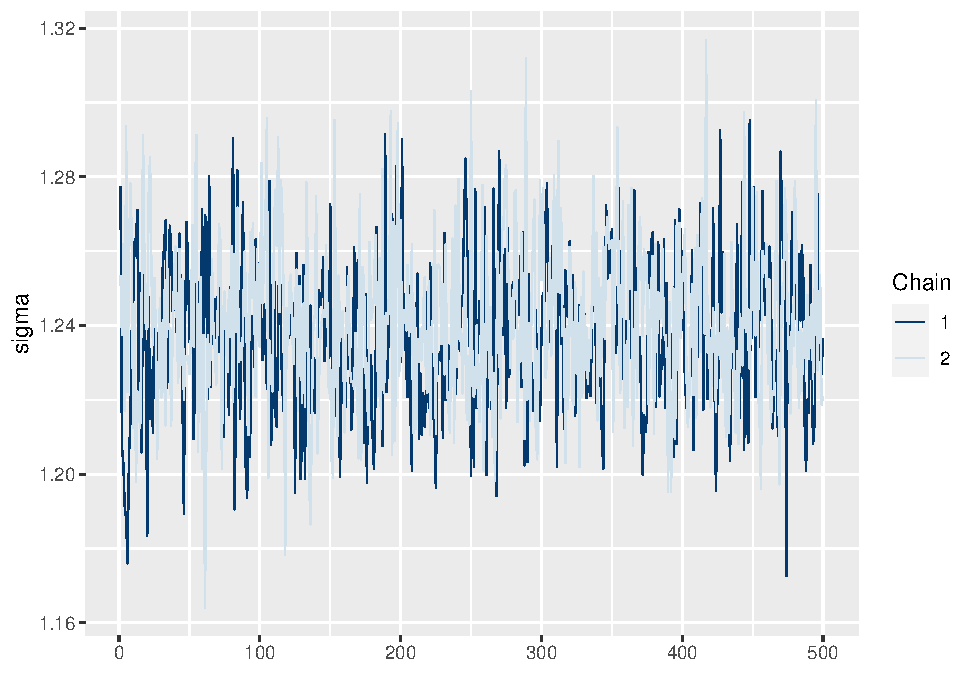
\includegraphics[width=0.5\linewidth]{04-lec_files/figure-latex/bayesplot-1} \end{center}

\end{document}
